\chapter{Ước lượng mật độ bằng histogram}\label{ch:hist}
\section{Đếm trong ô rồi chia cho độ rộng}
Giả sử trước hết $X_i\in[0,1]$, phân phối có mật độ $f$ trên miền này.
Chia thành $m$ ô bằng nhau, $h=1/m$:
\[
B_j=[(j-1)h,jh),\quad j<m,\qquad B_m=[(m-1)h,1].
\]
Quy ước ô trái đóng, phải mở, ngoại trừ ô cuối, đảm bảo mỗi quan sát được
đếm đúng một lần. Đặt
\[
N_j=\sum_i\1_{\{X_i\in B_j\}},\quad
p_j=\int_{B_j}f(u)\,du,\quad \widehat p_j=N_j/n.
\]
Histogram ước lượng mật độ là
\[
\boxed{\widehat f_{\rm hist}(x)=\frac{\widehat p_j}{h}
=\frac{N_j}{nh},\quad x\in B_j,}
\]
và bằng 0 ngoài $[0,1]$. $p_j/h$ là chiều cao trung bình thật trong ô;
$\widehat p_j/h$ mới là ước lượng từ mẫu.

\step{Kiểm tra là mật độ.}
Chiều cao không âm. Vì diện tích của ô $j$ là chiều cao nhân chiều rộng,
\[
\int\widehat f_{\rm hist}(x)\,dx
=\sum_{j=1}^m\frac{N_j}{nh}h
=\frac1n\sum_jN_j=1.
\]
Trên $[a,b]$, dùng $h=(b-a)/m$, trung điểm
$c_j=a+(j-1/2)h$. Nếu chuyển $U=(X-a)/(b-a)$ về $[0,1]$,
thì mật độ gốc phải là $\widehat f_X(x)=\widehat f_U((x-a)/(b-a))/(b-a)$.
Không thiếu hệ số Jacobian này.
\intuition{Chiều cao histogram là ``xác suất trong ô trên mỗi đơn vị độ dài''.
Biểu đồ số đếm chỉ có chiều cao $N_j$ chưa phải mật độ chuẩn hóa.}
\source{\cite{slide2}, slide 12; \cite{wasserman}, Mục 6.2}

\section{Kỳ vọng và phương sai chính xác}
Mỗi $N_j\sim\operatorname{Binomial}(n,p_j)$, dù các số đếm giữa ô khác
nhau không độc lập. Với $x\in B_j$,
\[
\E\widehat f_{\rm hist}(x)=\frac{p_j}{h},\qquad
\boxed{\Var\widehat f_{\rm hist}(x)=\frac{p_j(1-p_j)}{nh^2}.}
\]
Từ $\Var N_j=np_j(1-p_j)$, chỉ cần chia cho $(nh)^2$.
Kỳ vọng không phải $f(x)$ nói chung: estimator lấy trung bình mật độ
trong ô chứ không khôi phục biến thiên bên trong ô.

\section{Taylor và độ chệch tại một điểm}
Giả sử $f\in C^2([0,1])$, các đạo hàm được hiểu một phía ở biên.
Với $u,x\in B_j$ và $\norm{f''}_\infty<\infty$,
\[
f(u)=f(x)+f'(x)(u-x)+O((u-x)^2).
\]
Vì $|u-x|\leq h$, tích phân phần dư trên một ô có độ dài $h$ là $O(h^3)$.
Đặt $c_j=(j-1/2)h$:
\begin{align*}
p_j&=hf(x)+f'(x)\int_{(j-1)h}^{jh}(u-x)\,du+O(h^3)\\
&=hf(x)+hf'(x)(c_j-x)+O(h^3),
\end{align*}
vì trung bình của $u$ trên ô là $c_j$.
Chia cho $h$, rồi trừ $f(x)$, nhận
\[
\boxed{\Bias(\widehat f_{\rm hist}(x))
=f'(x)(c_j-x)+O(h^2)=O(h).}
\]
Tại đúng trung điểm $x=c_j$, số hạng bậc nhất mất. Taylor quanh $c_j$
còn cho $p_j/h-f(c_j)=h^2f''(c_j)/24+o(h^2)$.
Đây là cải thiện ở trung điểm, không phải bias $O(h^2)$ cho toàn histogram.

Thế $p_j=hf(x)+O(h^2)$ vào phương sai:
\[
\frac{p_j(1-p_j)}{nh^2}
=\frac{f(x)}{nh}+O(1/n).
\]
Nếu $f(x)>0$, số hạng chính là $f(x)/(nh)$; nếu $f(x)=0$, không thể
hiểu ký hiệu xấp xỉ theo tỷ số với số hạng chính bằng 0.
Khi $h\to0$, $nh\to\infty$, bias và variance cùng về 0, nên histogram
nhất quán theo MSE tại những điểm thỏa điều kiện trên.
\intuition{Ở ô có mật độ tăng, trung bình ô lớn hơn giá trị bên trái và
nhỏ hơn giá trị bên phải. Dấu chệch phụ thuộc vị trí của $x$ so với trung
điểm, không chỉ phụ thuộc độ dốc.}
\source{\cite{slide2}, slide 13--14; \cite{wasserman}, trang in 128--129,
phụ lục chứng minh trang in 140--142 (PDF 149--151)}

\section{Từ sai số tại điểm đến MISE}
\subsection{Tích phân bình phương chệch: nguồn gốc 1/12}
Trong ô $B_j$, có thể viết đều theo $x$:
$b(x)=f'(c_j)(c_j-x)+O(h^2)$.
Khi bình phương, hạng chéo được chặn bởi $O(h^3)$ tại điểm;
tích phân qua $m=1/h$ ô tổng độ dài 1 cho phần dư $O(h^3)$.
\begin{align*}
\int_0^1b(x)^2\,dx
&=\sum_j f'(c_j)^2\int_{B_j}(c_j-x)^2\,dx+O(h^3)\\
&=\sum_j f'(c_j)^2\int_{-h/2}^{h/2}t^2\,dt+O(h^3)\\
&=\frac{h^3}{12}\sum_j f'(c_j)^2+O(h^3)\\
&=\frac{h^2}{12}\int_0^1f'(x)^2\,dx+o(h^2).
\end{align*}
Ở bước hai, đặt $t=x-c_j$, $dx=dt$. Bước ba dùng
$[t^3/3]_{-h/2}^{h/2}=h^3/12$. Bước cuối dùng hội tụ tổng Riemann
$h\sum_j f'(c_j)^2\to\int_0^1f'^2$.

\subsection{Phương sai tích phân: công thức chính xác}
Phương sai là hằng trong mỗi ô, nên
\begin{align*}
\int_0^1\Var\widehat f_{\rm hist}(x)\,dx
&=\sum_jh\frac{p_j(1-p_j)}{nh^2}\\
&=\frac1{nh}\left(\sum_jp_j-\sum_jp_j^2\right)\\
&=\boxed{\frac1{nh}\left(1-\sum_jp_j^2\right)}.
\end{align*}
Với $f$ liên tục, $p_j=hf(\xi_j)$ cho một $\xi_j\in B_j$;
$\sum_jp_j^2/h=h\sum_j f(\xi_j)^2\to\int_0^1 f^2$.
Vậy phương sai tích phân bằng
\[
\frac1{nh}-\frac1n\int_0^1f(x)^2\,dx+o(1/n).
\]
Số hạng $-R(f)/n$ có bậc nhỏ hơn $1/(nh)$ khi $h\to0$;
nó không bằng 0 trong công thức chính xác.

\subsection{Băng thông và tốc độ tối ưu}
Đặt $A=\int_0^1f'^2>0$. Biểu thức tiệm cận chính là
\[
\AMISE_{\rm hist}(h)=\frac{A}{12}h^2+\frac1{nh}.
\]
Đạo hàm bằng $Ah/6-1/(nh^2)$, nên
\[
\boxed{h_*=(6/A)^{1/3}n^{-1/3},\qquad
\AMISE_{\rm hist}(h_*)=
\frac{6^{2/3}}4 A^{1/3}n^{-2/3}.}
\]
Để kiểm tra hệ số, tại nghiệm $1/(nh_*)=Ah_*^2/6$, bằng hai lần
phần bình phương chệch. Tổng bằng $Ah_*^2/4$.
Với $h=1/m$, chọn số nguyên $m$ gần $1/h_*$, so sánh hai ứng viên
lân cận. Nếu $A=0$, công thức suy biến: với mật độ đều trên miền biết
trước $[0,1]$, một ô duy nhất cho mật độ đúng bằng 1, rủi ro 0.

\begin{example}
Với $f(x)=2x$ trên $[0,1]$, $A=4$, nên
$h_*=(3/(2n))^{1/3}$. Nếu $n=96$, $h_*=1/4$, $m=4$.
Phần bình phương chệch chính là $1/48$, phương sai chính $1/24$,
tổng $1/16$. Đây là AMISE, không phải MISE chính xác.
\end{example}
\intuition{Ô rộng giảm dao động số đếm nhưng làm mất độ dốc bên trong ô.
Ở tối ưu, hai thành phần có cùng bậc theo $n$, nhưng không bằng nhau
về hằng số. Histogram đạt $n^{-2/3}$ dưới điều kiện đang xét.}
\source{\cite{slide2}, slide 15--16; \cite{wasserman}, Mục 6.2}

\section{Leave-one-out cross-validation}
Ta muốn chọn $h$ mà không biết $A$. Khai triển mất mát của một mẫu:
\[
\ISE(h)=\int\widehat f_h^2-2\int\widehat f_h f+R(f).
\]
Hạng $R(f)$ không phụ thuộc $h$, nên bỏ khi tối ưu.
Thay $\int\widehat f_h f$ bằng trung bình leave-one-out:
\[
\widehat J(h)=\int\widehat f_h^2(x)\,dx
-\frac2n\sum_i\widehat f_{(-i),h}(X_i).
\]
Giữ \emph{cùng phân hoạch} khi bỏ quan sát, chỉ đổi số đếm và mẫu số.
Nếu $X_i\in B_j$, $\widehat f_{(-i),h}(X_i)=(N_j-1)/((n-1)h)$.
Do đó
\begin{align*}
\int\widehat f_h^2&=\frac1{n^2h}\sum_jN_j^2,\\
\frac2n\sum_i\widehat f_{(-i),h}(X_i)
&=\frac2{n(n-1)h}\sum_jN_j(N_j-1)\\
&=\frac2{n(n-1)h}\left(\sum_jN_j^2-n\right).
\end{align*}
Trừ hai dòng, đổi $N_j^2=n^2\widehat p_j^2$:
\[
\boxed{\widehat J(h)=\frac2{(n-1)h}
-\frac{n+1}{(n-1)h}\sum_j\widehat p_j^2.}
\]
Với phân hoạch cố định, $\E\widehat f_{(-i),h}(x)=p_j/h=
\E\widehat f_{n,h}(x)$ trên ô $j$. Vì $X_i$ độc lập với mẫu bỏ $i$,
\[
\E\widehat f_{(-i),h}(X_i)
=\int\E\widehat f_{(-i),h}(x)f(x)\,dx
=\E\int\widehat f_{n,h}(x)f(x)\,dx.
\]
Suy ra $\E\widehat J(h)=\MISE_n(h)-R(f)$.
Phần bình phương đầu dùng estimator cỡ mẫu $n$; không tự thay tất cả
thành estimator cỡ mẫu $n-1$.

\begin{example}
Mẫu $(0.1,0.2,0.4,0.8)$, ứng viên $m=2,4$.
Với $m=2$, số đếm $(3,1)$ và $\sum\widehat p_j^2=10/16$:
\[
\widehat J(1/2)=\frac2{3/2}-\frac5{3/2}\frac{10}{16}=-\frac34.
\]
Với $m=4$, số đếm $(2,1,0,1)$ và $\sum\widehat p_j^2=6/16$:
\[
\widehat J(1/4)=\frac2{3/4}-\frac5{3/4}\frac6{16}=\frac16.
\]
Chọn $m=2$ trong hai ứng viên. Điểm CV âm là bình thường vì nó ước lượng
MISE trừ một hằng số dương.
\end{example}
\pitfall{Nếu dùng chính $X_i$ để đánh giá mật độ có chứa nó, quan sát tự
đóng góp vào mật độ và làm thiên lệch tiêu chuẩn. Nếu chọn gốc ô từ mẫu,
chứng minh không chệch cho phân hoạch cố định không còn áp dụng nguyên xi.}
\intuition{CV dùng một quan sát làm điểm đánh giá cho mô hình học từ
những quan sát còn lại. Mục tiêu là tối ưu rủi ro, không phải làm đường
cong trông đẹp nhất bằng mắt.}
\source{\cite{slide2}, slide 17; \cite{wasserman}, Mục 6.1--6.2}

\section{Bốn hạn chế cốt lõi}
\begin{enumerate}
\item \textbf{Không liên tục.} Đường mật độ nhảy ở ranh giới ô; không phù
hợp nếu muốn đạo hàm trơn hoặc vị trí đỉnh ổn định.
\item \textbf{Nhạy với gốc chia ô.} Dịch phân hoạch có thể làm một đỉnh
bị tách hoặc gộp dù dữ liệu và độ rộng ô không đổi.
\item \textbf{Khả năng tận dụng độ trơn hạn chế.} Với hàm có độ dốc,
bias thường $O(h)$, tốc độ MISE $n^{-2/3}$, chậm hơn KDE bậc hai
trong lớp mật độ đủ trơn và điều kiện biên phù hợp.
\item \textbf{Khó mở rộng theo số chiều.} Với ô lập phương cạnh $h$,
số ô tăng như $h^{-d}$, dữ liệu trong mỗi ô ít đi; phương sai có bậc
$1/(nh^d)$.
\end{enumerate}
\begin{figure}[htbp]
\centering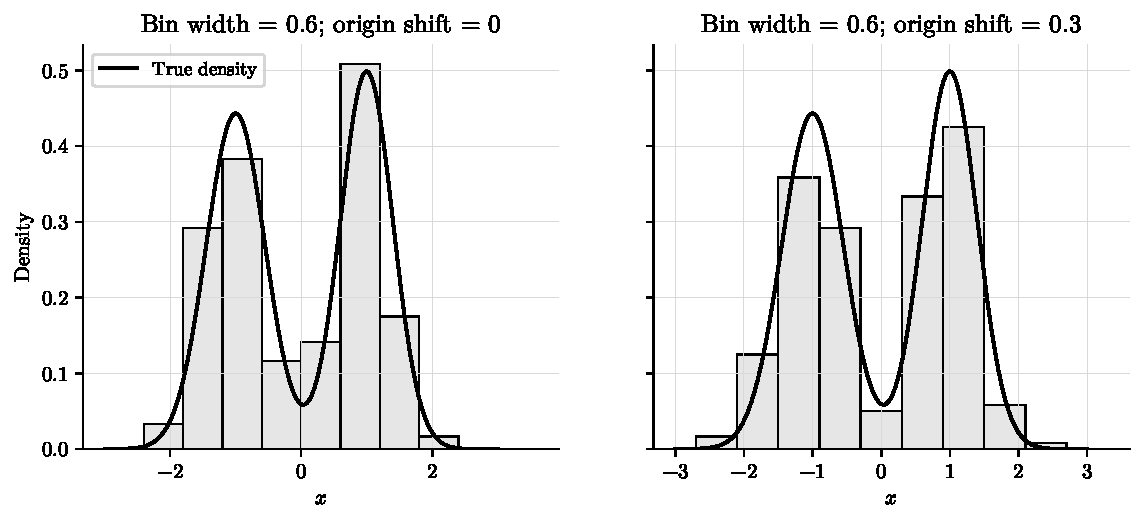
\includegraphics[width=.95\textwidth]{hist_origin.pdf}
\caption{Cùng mẫu và độ rộng ô, hai gốc chia ô khác nhau cho hai histogram.
Đường liền là mật độ hỗn hợp thật. Hình dùng ô trên toàn trục để minh họa
độ nhạy với gốc, khác thiết lập $h=1/m$ trên $[0,1]$ của phần chứng minh.}
\end{figure}
\intuition{KDE thay việc gán toàn bộ khối lượng vào một ô bằng việc đặt
một bản kernel quanh mỗi quan sát. Điều này loại bỏ gốc lưới cố định;
mức độ trơn vẫn phụ thuộc kernel được chọn.}
\source{\cite{slide2}, slide 18}
